\documentclass[a4paper, 12pt]{article}

\usepackage[utf8]{inputenc}
\usepackage[T1]{fontenc}
\usepackage[french]{babel} 
\usepackage[top=35mm, bottom=35mm, left=25mm, right=25mm]{geometry}
\usepackage{geometry}
\usepackage{graphicx}
\usepackage{multirow}  
\usepackage{subfigure}
\usepackage{verbatim}
\usepackage{url}
\usepackage{algorithmic, algorithm} 
\usepackage{amsmath,amsfonts,amssymb}
\usepackage{lmodern}
\usepackage{microtype}
\usepackage{xcolor}
\usepackage{textcomp}
\usepackage{minted}
\usepackage{framed}
\usepackage{tcolorbox}
\usepackage{etoolbox}
\BeforeBeginEnvironment{minted}{\begin{tcolorbox}[left=8mm]\begin{center}}
\AfterEndEnvironment{minted}{\end{center}\end{tcolorbox}}%
\usepackage{hyperref}
\hypersetup{
    colorlinks,
    citecolor=blue,
    filecolor=black,
    linkcolor=magenta,
    urlcolor=blue,
}
\hypersetup{
pdfpagemode={},
pdfstartview={XYZ 3000 3000 0.75}
pdfstartview={XYZ left top zoom}
}
\hypersetup{
pdftitle={Template de rapport \LaTeX},
pdfsubject={Sujet du rapport, peut être vide},
pdfauthor={Premier auteur et Deuxième auteur},
pdfkeywords = {Premier mot clé, Deuxième mot clé, etc...}
}
\setcounter{secnumdepth}{3}
\usepackage{fancyhdr}
\pagestyle{fancy}
 \lhead{\leftmark}
 \rhead{}
\usepackage{pgf, tikz}
\usetikzlibrary{arrows}


\newcommand{\makelogos}{
\begin{tikzpicture}[remember picture,overlay]
\node [shift={(3 cm,-2cm)}]  at (current page.north west){

\includegraphics[scale=.25]{images/insacvl.png}
};
\node [shift={(-3.675 cm,-2cm)}]  at (current page.north east){
\begin{minipage}{.01\textwidth}
\rotatebox{90}{\scalebox{.75}{Département}~~~~}
\end{minipage}
};
\node [shift={(-3 cm,-2cm)}]  at (current page.north east){
\begin{minipage}{.1\textwidth}
\hspace{-.5cm}
\begin{eqnarray}
&\textbf{{\color{red}S}}&\!\!\!\!\!\textnormal{écurité et}\nonumber\\
&\textbf{{\color{red}T}}&\!\!\!\!\!\textnormal{echnologies}\nonumber\\
&\textbf{{\color{red}I}}&\!\!\!\!\!\!\textnormal{nformatiques}\nonumber
\end{eqnarray}
\end{minipage}
};
\end{tikzpicture}
}
 % A priori, vous n'aurez pas besoin de modifier le contenu de ce fichier :)


\begin{document}
\pagenumbering{roman} 

%%% Remarque sur la page de garde :
% Il existe une commande beaucoup plus simple : \maketitle
% Cette commande ne permet pas directement l'insertion de logo et de données 
% additionnelles sans modifier certains fichiers de configuration
% (utilisation avancée)

\begin{titlepage}
\setlength{\headheight}{0cm}
\setlength{\headsep}{0cm}
{

%%% Insertion des logos [begin]
\makelogos
%%% Insertion des logos [end]

\vspace{4cm}

\begin{center}
\fbox{ 
\begin{minipage}[h]{.9\linewidth}
\begin{center}
{\vspace*{5mm}
\huge\textbf{Rapport Ouverture Scientifique et Technique}\\  %%% Titre du rapport
\vspace*{5mm}}
\end{center}
\end{minipage}
}

\vspace{15mm}

Auteur\\~\\
{\large 
\bsc{Dubois} Louan\\
\bsc{Maachi} Kaoutar\\
\bsc{Techer} Luc}\\
~\\
\underline{STI, 4A}\\ 

\vspace{3cm}  

\textbf{Année Universitaire 2020 - 2021\\
{\tiny version : \today}}

\vspace{2cm}  

\end{center}
  
\vfill

\begin{flushleft}
	Encadrant : \textsc{Toinard} Christian
\end{flushleft}

}
\end{titlepage}

\newpage		
\tableofcontents % Insertion de la table des matières
\addcontentsline{toc}{section}{Table des matières}

% Vous pouvez également pour des rapports plus longs (des rapports de stages par exemple) insérer une table des figures
%\listoffigures
%\addcontentsline{toc}{section}{Liste des figures} 

% Voir même une liste des algorithmes
%\listofalgorithms
%\addcontentsline{toc}{section}{Liste des algorithmes}

\clearpage 

\pagenumbering{arabic}

\section{Contexte}
Les processeurs, dont l’évolution a été caractérisée par une augmentation continue de la fréquence de fonctionnement, suivent depuis quelques années une nouvelle voie, celle du multi-coeur.
Les limites acceptables étant atteintes, la multiplication des processeurs dans un même système offre une autre possibilité d’augmentation de la puissance de calcul.
\newline 
Un système d'exploitation est principalement composé d'un noyau. Celui-ci est une couche d'abstraction entre le matériel (processeur, mémoire) et le logiciel (application, \emph{user space}), et permet leur communication. Il peut être monolithique, c'est-à-dire un programme qui est tel qu'il est et ne peut pas être modifié, pas d'ajout de fonctionnalités possible sans le recompiler. Il peut également être modulaire, qui signifie que l'on peut lui ajouter des programmes qui étendent ses fonctionnalités, et aussi les supprimer.
\newline
d'autre part le microkernel est un logiciel ou un code qui contient le minimum requis de fonctions, de données et de fonctionnalités pour implémenter un système d'exploitation. Il fournit un nombre minimal de mécanismes, ce qui est assez bon pour exécuter les fonctions les plus élémentaires d'un système d'exploitation. Il permet à d'autres parties du système d'exploitation d'être implémentées car il n'impose pas beaucoup de politiques.
\newline
Un Microkernel est la partie la plus importante pour une implémentation correcte d'un système d'exploitation, on peut voir dans le diagramme ci-dessous, que Microkernel accomplit des opérations de base comme la mémoire, les mécanismes de planification de processus et la communication inter-processus.
   \begin{figure}[h]
\centering
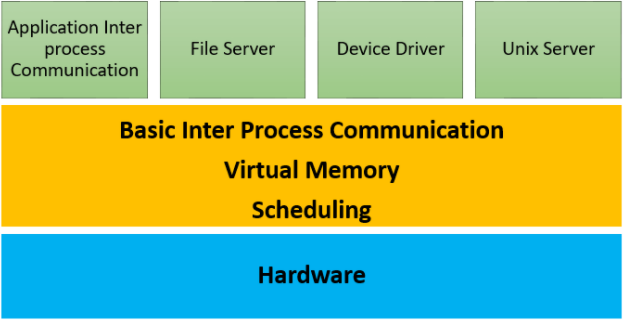
\includegraphics[scale=0.5]{image2.PNG}
\caption{Microkernel Based Operating System}
\end{figure}
\newline
Distributed computing est une technologie beaucoup plus large qui existe depuis plus de trois décennies de maintenant. En termes simples, il est un calcul sur des ordinateurs autonomes distribués qui ne communiquent que sur un réseau, ces systèmes sont généralement traités différemment des systèmes informatiques parallèles ou des systèmes à mémoire partagée, où plusieurs ordinateurs partagent un pool de mémoire commun utilisé pour la communication entre les processeurs. Les systèmes de mémoire distribuée utilisent plusieurs ordinateurs pour résoudre un problème commun, le calcul étant réparti entre les ordinateurs connectés (nœuds) et utilisant la transmission de messages pour communiquer entre les nœuds. Par exemple, le calcul en grille est une forme de calcul distribué où les nœuds peuvent appartenir à différents domaines administratifs. Un autre exemple est la solution de virtualisation du stockage en réseau qui utilise le calcul distribué entre des serveurs de données et de métadonnées.
   \begin{figure}[h]
\centering
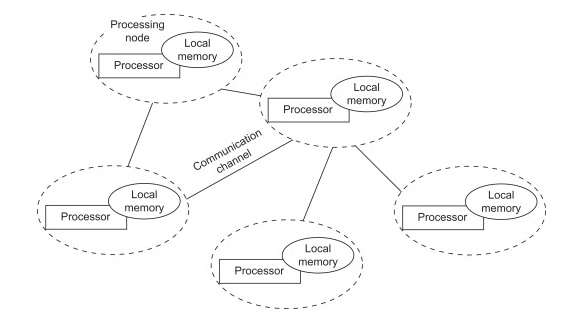
\includegraphics[scale=0.5]{image3.PNG}
\caption{A distributed computing system}
\end{figure}
\newline


\clearpage 
\section{Problématique}

Dans les années 1990, tous les systèmes d'exploitation étaient basés sur des noyaux monolithiques ce qui limitait grandement les possibilités de développement de systèmes en rendant compliqué l'intégration de tels noyaux sur des architectures matérielles complexes, ils n'ont pas réussi à fournir aux développeurs d'applications une flexibilité suffisante. Ils fournissent une foule d'abstractions inefficaces et souvent inappropriées qui empêchent les applications d'accéder au matériel pour exploiter les gains d'efficacité.\newline

Les développeurs avaient alors besoin d'un système d'exploitation fiable, sécurisé et modulable afin de pouvoir l'exploiter au mieux dans leurs applications. \\
De plus, un noyau monolithique limite la compatibilité et l'optimisation vis-à-vis d'architectures variées. A l'époque, les ordinateurs hautes performances et les super-ordinateurs possédaient plusieurs processeurs tandis que les ordinateurs grand-public n'en possaidaient qu'un. L'objectif de cette recherche était donc de créer un noyau modulaire qui pouvait être facilement adapté à différentes architectures plus ou moins complexes.

\clearpage 
\section{Apports scientifiques principaux de l’article}
\subsection{Le concept des micro-noyaux}
\paragraph{}

Dans cet article, le concept des micro-noyaux est introduit. Il s'agit d'une solution qui consiste à réduire au plus possible le noyau (aussi appelé Nucleus) afin que celui-ci ne puisse effectuer que des tâches élémentaires. Les autres fonctionnalités seront quant à elles effectuées par des serveurs modulaires. Ces serveurs sont en réalité des sous-systèmes qui pourront échanger des informations entre-eux en utilisant des Communications Inter-Processus (IPC). Ces différents sous-systèmes pourront alors être répartis sur un seul ou plusieurs processeurs ou machines. Afin de faciliter les communications entre les différents serveurs, l'article propose aussi la mise en place de Remote Procedure Call (RPC) qui est un protocole qui permet d'exécuter des commandes sur un serveur à distance. \\
La mise en place de micro-noyaux permettrait de faciliter grandement la répartition et l'isolations de différentes parties du systèmes sur des processeurs ou machines différentes tout en restant compatible avec des architectures plus simples. Ceci permettrait aussi aux développeur de pouvoir créer, tester et implémenter de nouvelles fonctionnalités beaucoup plus simplement.

\subsection{Présentation de Chorus}
\paragraph{}
Chorus est un système d'exploitation novateur pour l'époque créé par le laboratoire de recherche INRIA (France) puis développé d'avantage et commercialisé par CHORUS Systems. Il s'agit de l'exemple d'implémentation des micro-noyaux décrite dans l'article. A l'époque, c'était l'une des rare distribution à explorer le domaine des micro-noyaux avec quelques autres exemples notoires tels que Amoeba, Topaz et System-V. Chorus fut une distribution novatrice dont le développement a malheureusement été abandonné depuis. Cependant, Chorus a constitué une base solide pour le développement des micro-noyaux. L'architecture de Chorus est constituée, comme décrit précédemment, d'un micro-noyau qui peut effectuer des fonctionnalités élémentaires et de serveurs qui viennent compléter ce Nucleus.
\\
\paragraph{}
Chorus-v3 était une référence en la matière car il s'agissait de la 4$\sup{ème}$ génération de la distribution. De plus elle faisait usage de contributions de la part de System-V notament dans ce qui est des communications inter-processus et des RPC, de Mach pour ce qui est de la gestion de la mémoire virtuelle partagée et des threads, Amoeba pour la gestion d'addresse et les capacités de binding. Chorus a donc essayé de prendre le meilleur des différentes distributions existantes afin de créé une référence en terme de système d'exploitation utilisant les micro-noyaux.
\\
\paragraph{}
Le Nucleus de Chorus est un noyau temps réel qui implémente le calcul distribué et les communications de bas niveau. Il est lui-même composé de 4 composants différents :
\begin{itemize}
	\item Un puissant ordonanceur permettant la gestion des différents processeurs et threads afin de pouvoir exécuter les tâches de manière optimisée et distribuée;
	\item Un gestionnaire de mémoire distribuée qui supporte toutes les architectures mémoires;
	\item Un superviseur d'évènement de bas niveau qui permet de distribuer les intéruptions système, trapes et exeptions venant de l'extérieur sur des ports ou routines définis dynamiquement;
	\item Un gestionnaire de communication inter-processus qui fournit d'excélentes performances de communications entre les différents services.
\end{itemize}

\paragraph{}
Les sous-systèmes utilisés par Chorus sont en quelques sortes des morceaux de systèmes d'exploitation conventionnels qui agissent par dessus le Nucleus. Ils permettent la gestion de ressources physiques et logiques telles que la gestions des fichiers, des gestionnaires de fichiers, des appareils ainsi que des communication de plus haut niveau. L'architecture est telle qu'un processus ne peut pas voir un sous-système comme un fragment du noyau mais bien comme un système d'exploitation standart. Ceci est dû aux interfaces proposées par les sous-systèmes qui doivent être rigoureusement les mêmes que celles offertes par un système classique. Chaque sous-système possède donc son interface qui interagit avec ses composants et le Nucleus. Cette architecture permet, en plus de faciliter la distribution du système, de grandement simplifier le développement système en faisant abstraction des fonctionnalités de très bas niveau étant donné qu'elles sont déjà implémentées dans le Nucleus.

\clearpage 
\section{Impacts de l'article}
\paragraph{}
L’article de recherche est un  ancien article qui est publié en janvier 1991 et il possède 13 citations sur Google scholar en mars 2021.
\newline 
Ce qu'il faut savoir a propos de ses auteurs c'est que "Michel Gien" c'est un co-founder & CTO of Chorus Systems, il a dirigé la direction technique du système d'exploitation Chorus, pionnier dans la conception de systèmes d'exploitation basés sur des micro-noyaux et distribué UNIX par "image système unique" sur des architectures multi-ordinateurs ainsi que l'évolution de Chorus vers un système d'exploitation distribué évolutif en temps réel, il a évangélisé l'approche du système d'exploitation Chorus auprès de la communauté scientifique et des marchés commerciaux. il a continué à publier d'autres articles dans le même contexte de notre article par exemple on peut citer \cite{n1}.Ainsi, tout porte à croire que l'article a ouvert la voie à de nombreuses réflexions indépendantes sur le sujet . 
\paragraph{}
Notre article est très souvent cité comme outil majeur pour faire référence au micrkernel "CHORUS", parmi les articles qu'ils le cite on trouve par exemple \cite{n2} l'article qui parle de la comparaison des 3 microkernels au niveau de la gestion des processus, de la gestion de la mémoire et de la communication et cet article a été cité 23 fois d'où son impact qui est non negligeable.


 
\section{Analyse critique du travail proposé}
\paragraph{}
L'article proposé fait un état de l'art partiel en ce qui concerne les micro-noyaux. Sa construction semble logique, en introduisant dans un premier temps ce qu'est un micro-noyau puis dans un second temps en présentant un exemple représentatif d'implémentation. Il évoque à plusieurs reprises d'autres travaux tels que Amoeba, Topaz, System-V, MOS ou encore  Mach, ce qui contribue à l'aspect "état de l'art" de l'article. Cependant l'article est principalement orienté vers la description de Chorus spécifiquement. De plus, le point de vue des auteurs semble être biaisé en faveur du système Chorus qui ne rencontre presque aucune critique négative. On peut donc peut-être questionner l'intégrité scientifique des auteurs dans cet article.
\paragraph{}
Les enjeux éthiques présentés dans cet article sont majoritairement concentrés sur le souhait de progrès et la facilitation du développement système. En effet, les micro-noyaux offrent une solution à la difficulté croissante du développement système en proposant un système d'API noyau. Cet article présente des avancées majeures dans ce domaine qui sont suffisemment et relativement simplement expliquées afin de pouvoir être assimilées par tout un chacun. L'objectif principal de cet article est donc la vulgarisation de ces avancées. \paragraph{}
Les micro-noyaux présentent aussi des avantages en matière de sécurité étant donné que les différentes composantes du système sont isolées. La diffusion de ces connaissances permet donc aussi, de manière indirecte, de participer à l'amélioration de la sécurité globale des systèmes.
\paragraph{}
Dans sa conclusion, l'article laisse penser que les micro-noyaux deviendraient probablement une partie essentielle des systèmes modernes ce qui est une excellente prédiction étant donné qu'ils sont maintenant utilisés dans plusieurs systèmes d'exploitation grand public.

\clearpage 
\section*{Conclusion}
\addcontentsline{toc}{section}{Conclusion}

Ce projet nous a permis, outre de nous familiariser avec \LaTeX{}, d'en apprendre plus sur le fonctionnement concret des micro-noyaux. Il s'agissait pour l'époque d'une technologie novatrice qui est aujourd'hui très présente dans les différents systèmes d'exploitation modernes. Il s'agissait aussi d'une première introduction intéressante à la lecture de papiers scientifiques. Pour certains d'entre nous, nous en avions déjà rencontrés quelques-uns lors de notre projet du semestre 7. Cependant c'est la première fois que nous pouvons constater l'impact réel qu'a pu avoir un tel article sur la communauté du développement informatique. C'était aussi une bonne occasion de réfléchir sur les enjeux et les conséquences éthiques d'un article scientifique.

\clearpage 
\bibliographystyle{plain}
\bibliography{bibliographie}
\addcontentsline{toc}{section}{Références}


\clearpage 
\appendix
\end{document}
